\documentclass[11pt,a4paper]{article}

% === Font & encoding (XeLaTeX + xeCJK) ===
\usepackage{fontspec}
\setmainfont{Latin Modern Roman}
\setsansfont{Latin Modern Sans}
\setmonofont{Latin Modern Mono}

\usepackage{xeCJK}
\setCJKmainfont{Noto Sans CJK KR}
\setCJKsansfont{Noto Sans CJK KR}
\setCJKmonofont{Noto Sans CJK KR}

% === Paragraph style ===
\setlength{\parindent}{1.5em}
\setlength{\parskip}{0.4em}

% === Layout ===
\usepackage[margin=2cm,headheight=14pt]{geometry}
\usepackage{graphicx}
\usepackage{booktabs}
\usepackage{longtable}
\usepackage{float}
\usepackage{hyperref}
\usepackage{xcolor}
\usepackage{fancyhdr}
\usepackage{titlesec}
\usepackage{caption}
\usepackage{multirow}
\usepackage{enumitem}
\usepackage{array}
\usepackage{tabularx}
\usepackage{amssymb}
\usepackage[normalem]{ulem}

% === Header/Footer ===
\pagestyle{fancy}
\fancyhf{}
\rhead{Cross-Model SAE Analysis}
\lhead{LLM Gambling Addiction}
\cfoot{\thepage}

% === Section styling ===
\titleformat{\section}{\Large\bfseries}{\thesection}{1em}{}
\titleformat{\subsection}{\large\bfseries}{\thesubsection}{1em}{}
\titleformat{\subsubsection}{\normalsize\bfseries}{\thesubsubsection}{1em}{}

% === Hyperlinks ===
\hypersetup{
    colorlinks=true,
    linkcolor=blue!60!black,
    citecolor=green!50!black,
    urlcolor=blue!70!black
}

% === Title ===
\title{\textbf{LLM의 위험 의사결정에 대한\\교차 모델, 교차 도메인 신경 기반 분석}\\[0.3em]
\normalsize ``대규모 언어 모델은 도박 중독에 걸릴 수 있는가?''}
\author{이승필, 신동현, 이윤정, 김선동\\
\small GIST (광주과학기술원)}
\date{2026년 3월 25일}

\begin{document}
\maketitle
\tableofcontents
\newpage

% ============================================================
% 개요
% ============================================================
\section*{개요}
\addcontentsline{toc}{section}{개요}

대규모 언어 모델(Large Language Model)이 도박 과제에서 파산(bankruptcy)할 때---잔고가 0이 될 때까지 반복적으로 베팅을 선택할 때---네트워크 내부에서는 무엇이 일어나는가? 본 보고서는 이 내부 ``파산 신호(bankruptcy signal)''가 서로 다른 모델, 도박 도메인, 실험 조건에 걸쳐 공유되는 보편적 속성인지, 아니면 각 설정마다 고유한 신경 패턴을 생성하는지를 묻는다.

두 개의 트랜스포머(Transformer) 모델을 분석한다: \textbf{Gemma-2-9B-IT} (Google, 42층, 3{,}584차원)과 \textbf{LLaMA-3.1-8B-Instruct} (Meta, 32층, 4{,}096차원). 각 모델은 세 가지 음의 기대값 도박 패러다임---투자 선택(Investment Choice, IC), 슬롯 머신(Slot Machine, SM), 미스터리 휠(Mystery Wheel, MW)---을 수행하며, 6개 모델--패러다임 조합에 걸쳐 총 16{,}000개 게임을 진행한다. 베팅 조건(고정/가변)과 프롬프트 구성요소(목표, 자금, 경고, 힌트, 페르소나)를 체계적으로 조작한다.

내부 표상(internal representation)은 두 수준에서 검토한다. \textbf{은닉 상태(Hidden states)}는 각 트랜스포머 층의 전체 활성화 벡터를 포착한다. \textbf{SAE 특징(SAE features)}은 이 은닉 상태의 희소하고 해석 가능한 분해로, GemmaScope (131K 특징/층)와 LlamaScope (32K 특징/층)를 통해 추출된다. 분류에는 StandardScaler $\rightarrow$ PCA(50) $\rightarrow$ 로지스틱 회귀(Logistic Regression, 균형 가중치, $C$=1.0)와 5-fold 층화 교차검증을 사용한다. 전이 AUC(Transfer AUC)에 200회 순열 검정(permutation test)을 적용하여 통계적 유의성을 확인한다.

\textbf{세 가지 연구 질문}:
\begin{itemize}[nosep]
    \item \textbf{RQ1}: Gemma와 LLaMA는 공통된 파산(BK) 패턴을 공유하는가?
    \item \textbf{RQ2}: 도박 도메인이 바뀌어도 BK 패턴이 유지되는가?
    \item \textbf{RQ3}: 베팅 조건이 바뀌어도 BK 패턴이 유지되는가?
\end{itemize}

V11은 V10을 두 가지 새로운 분석으로 확장한다: (1) 분류 파이프라인의 강건성 검증(PCA 차원 민감도 및 분류기 비교), (2) LLaMA에서의 BK 방향 조향(steering)을 통한 인과적 검증.

\bigskip\hrule\bigskip

% ============================================================
% 요약
% ============================================================
\section*{핵심 요약}
\addcontentsline{toc}{section}{핵심 요약}

\textbf{RQ1---두 모델 모두 거의 동일한 정확도와 균형 잡힌 신경 구조로 파산을 인코딩한다.} Gemma와 LLaMA는 모든 패러다임에서 BK 분류 AUC 차이가 0.006 이내이다 (0.954--0.976). L22에서 Gemma는 600개, LLaMA는 1{,}334개의 보편적 BK 뉴런을 가지며, 촉진(promoting)과 억제(inhibiting) 뉴런의 수가 대략 동일하다. 베팅 유형과 패러다임을 통제한 후에도 SAE 특징의 65--76\%가 BK에 유의하다 (순열 검정 $p$=0.000 vs 귀무 가설 ${\sim}$1\%).

\textbf{RQ2---한 도메인에서 훈련된 BK 분류기가 다른 도메인의 파산을 예측한다.} Gemma IC$\rightarrow$MW 전이 AUC 0.932 (L18); LLaMA MW$\rightarrow$IC 0.805 (L25). 두 모델 모두 거의 직교하는 패러다임별 가중치 벡터(코사인 $\approx$ 0.04)에도 불구하고 이를 달성하며, BK 신호가 단일 방향이 아닌 공유된 저차원 부분공간(subspace)을 차지함을 시사한다.

\textbf{RQ3---고정 베팅 파산으로 훈련된 분류기가 가변 베팅 파산을 예측하며, 그 반대도 성립한다.} 교차 베팅 유형 전이는 모든 LLaMA 층에서 AUC 0.74--0.93을 산출한다 (모두 $p$=0.000). Gemma SAE도 심층에서 이 패턴을 확인한다 (L30: 0.902). 415개 SAE 특징이 두 베팅 조건 모두에서 일관된 BK 효과를 보인다 (동일 부호, $d$$\geq$0.3).

\textbf{강건성---분류 결과는 PCA 차원 수와 분류기 선택에 둔감하다.} 6개 데이터셋 중 4개에서 AUC가 PCA=50에서 포화되며, 나머지 2개에서는 PCA=50이 PCA 미적용보다 우수하다 (BK 표본이 적어 과적합 가능성이 높은 경우). 로지스틱 회귀, MLP, SVM-RBF 간 AUC 차이가 모든 6개 데이터셋에서 0.007 이내로, BK 표상의 선형 분리 가능성(linear separability)을 확인한다.

\textbf{인과적 검증---BK 방향 벡터가 LLaMA의 도박 행동에 인과적 영향을 미친다.} L22의 잔차 스트림(residual stream)에 BK 방향을 추가하면 단조적 용량-반응(dose-response)이 나타난다: BK 비율이 34\% ($\alpha$=$-$2)에서 52\% ($\alpha$=$+$2)로 증가하며, Spearman $\rho$=0.927 ($p$=0.003). 뉴런 수준 제거(ablation)는 유의한 효과를 보이지 않아, BK가 분산 표상(distributed representation)임을 확인한다. 무작위 방향 통제(random direction control)는 비특이적 교란 효과를 완전히 배제하기 위해 다중 알파 검정이 필요하다.

\bigskip\hrule\bigskip

% ============================================================
% 1. 실험 설계
% ============================================================
\section{실험 설계}

\subsection{데이터}

\begin{table}[H]
\centering
\caption{데이터셋 개요}
\begin{tabular}{llccc}
\toprule
\textbf{패러다임} & \textbf{모델} & \textbf{게임 수} & \textbf{BK} & \textbf{BK\%} \\
\midrule
IC & Gemma & 1{,}600 & 172 & 10.8\% \\
IC & LLaMA & 1{,}600 & 142 & 8.9\% \\
SM & Gemma & 3{,}200 & 87 & 2.7\% \\
SM & LLaMA & 3{,}200 & 1{,}164 & 36.4\% \\
MW & Gemma & 3{,}200 & 54 & 1.7\% \\
MW & LLaMA & 3{,}200 & 2{,}426 & 75.8\% \\
\bottomrule
\end{tabular}
\end{table}

각 패러다임은 2가지 베팅 유형(고정/가변)과 32가지 프롬프트 조합을 사용한다. IC는 추가로 베팅 제약(c10/c30/c50/c70)을 변형한다. SM과 MW에서 LLaMA의 BK 비율은 Gemma보다 13--44배 높으며, 이는 두 모델이 매우 다른 행동 전략을 채택하면서도 BK 정보를 동등한 정확도로 인코딩함을 의미한다 (\S\ref{sec:rq1_classification_ko} 참조).

\subsection{주요 정의}

\begin{description}[style=nextline, leftmargin=2em]
    \item[파산 (Bankruptcy, BK)] 누적 손실로 잔고가 \$0에 도달하는 것. 주요 결과 변수이다.
    \item[의사결정 시점 (Decision Point, DP)] 각 게임에서 모델이 베팅 또는 중단을 결정하는 최종 시점의 활성화 상태이다.
    \item[보편적 BK 뉴런 (Universal BK neuron)] 검사한 모든 패러다임에서 BK 결과와의 상관이 FDR-유의하고 (BH, $p$<0.01) 동일한 부호를 가진 뉴런이다.
    \item[교차 도메인 전이 (Cross-domain transfer)] 한 패러다임에서 BK 분류기를 훈련하고 다른 패러다임에서 테스트한다. 순열 검정 $p$<0.05에서 AUC $\gg$ 0.5이면 공유된 BK 구조를 시사한다.
    \item[교차 베팅 유형 전이 (Cross-bet-type transfer, F1)] 고정 베팅 게임에서 BK 분류기를 훈련하고 가변 베팅 게임에서 테스트한다 (및 그 반대).
    \item[BK 방향 벡터 (BK direction vector)] 특정 층에서 평균 BK 은닉 상태와 평균 Safe 은닉 상태의 차이. 조향(steering) 실험에 사용된다 (\S\ref{sec:steering_ko}).
\end{description}

\bigskip\hrule\bigskip

% ============================================================
% 2. RQ1
% ============================================================
\section{RQ1: 두 모델이 공통된 BK 패턴을 공유하는가?}

\subsection{BK 분류}\label{sec:rq1_classification_ko}

두 모델 모두 각각의 최적 층에서 세 패러다임 모두 BK 분류 AUC > 0.95를 달성한다.

\begin{table}[H]
\centering
\caption{BK 분류 AUC}
\begin{tabular}{lccc}
\toprule
\textbf{패러다임} & \textbf{Gemma} & \textbf{LLaMA} & \textbf{차이} \\
\midrule
SM & 0.976 (L20) & 0.974 (L8) & 0.002 \\
IC & 0.960 (L30) & 0.954 (L12) & 0.006 \\
MW & 0.966 (L30) & 0.963 (L16) & 0.003 \\
\bottomrule
\end{tabular}
\end{table}

두 모델의 최적 깊이는 다르다---Gemma는 L20--L30, LLaMA는 L8--L16---그러나 최고 AUC 값의 차이는 최대 0.006이다. 이는 LLaMA MW의 BK 비율(75.8\%)이 Gemma MW(1.7\%)보다 44배 높음에도 불구하고 성립한다. 분류 파이프라인은 균형 클래스 가중치를 사용하므로, 이 동등성은 기저율(base rate)의 인위적 산물이 아니다. BK 정보는 두 아키텍처 모두에서 비슷한 충실도로 존재한다.

\subsection{보편적 BK 뉴런}

\begin{table}[H]
\centering
\caption{보편적 BK 뉴런 (L22)}
\begin{tabular}{lcc}
\toprule
 & \textbf{Gemma (3-패러다임)} & \textbf{LLaMA (2-패러다임)} \\
\midrule
총 뉴런 수 & 3{,}584 & 4{,}096 \\
보편적 BK 뉴런 & 600 (16.7\%) & 1{,}334 (32.6\%) \\
촉진 / 억제 & 302 / 298 & 672 / 662 \\
\bottomrule
\end{tabular}
\end{table}

LLaMA의 더 높은 수는 주로 다른 우연 수준을 반영한다: 2-패러다임 부호 일관성은 50\% 우연 기저선인 반면, 3-패러다임은 25\%이다. 핵심 발견은 절대 수가 아니라 \textbf{균형 비율}이다: 두 모델 모두 검사한 모든 층(L8--L30)에서 촉진과 억제 뉴런의 수가 대략 동일하다. 이 양방향 구조는 BK-촉진 신호와 BK-억제 신호가 공존하는 ``밀기-당기기(push-pull)'' 메커니즘을 시사한다.

\subsection{요인 분해 (Factor Decomposition)}

각 SAE 특징에 대해 OLS 회귀(\texttt{feature $\sim$ outcome + bet\_type + paradigm})를 수행하여, 베팅 유형과 패러다임을 통제한 후 BK 결과가 독립적으로 기여하는지 검정한다.

\begin{table}[H]
\centering
\caption{결과-유의 특징}
\begin{tabular}{lcccc}
\toprule
\textbf{모델} & \textbf{패러다임} & \textbf{특징 수} & \textbf{결과-유의} & \textbf{순열 귀무} \\
\midrule
Gemma & IC+SM+MW & 581 & 65.2\% (379) & ${\sim}$1\% \\
LLaMA & IC+SM & 1{,}418 & 69.5\% (985) & ${\sim}$1\% \\
LLaMA & IC+SM+MW & 1{,}056 & 75.8\% (800) & ${\sim}$1\% \\
\bottomrule
\end{tabular}
\end{table}

LLaMA 내에서 MW를 세 번째 패러다임으로 추가하면 결과-유의 비율이 69.5\%에서 75.8\%로 증가하며, 이는 추가 도메인이 패러다임 특이적 잡음(noise)을 걸러내되 BK 신호를 희석하지 않음을 나타낸다. 세 분해 모두 순열 귀무 가설(${\sim}$1\%)을 60배 이상 초과한다.

\begin{figure}[H]
\centering
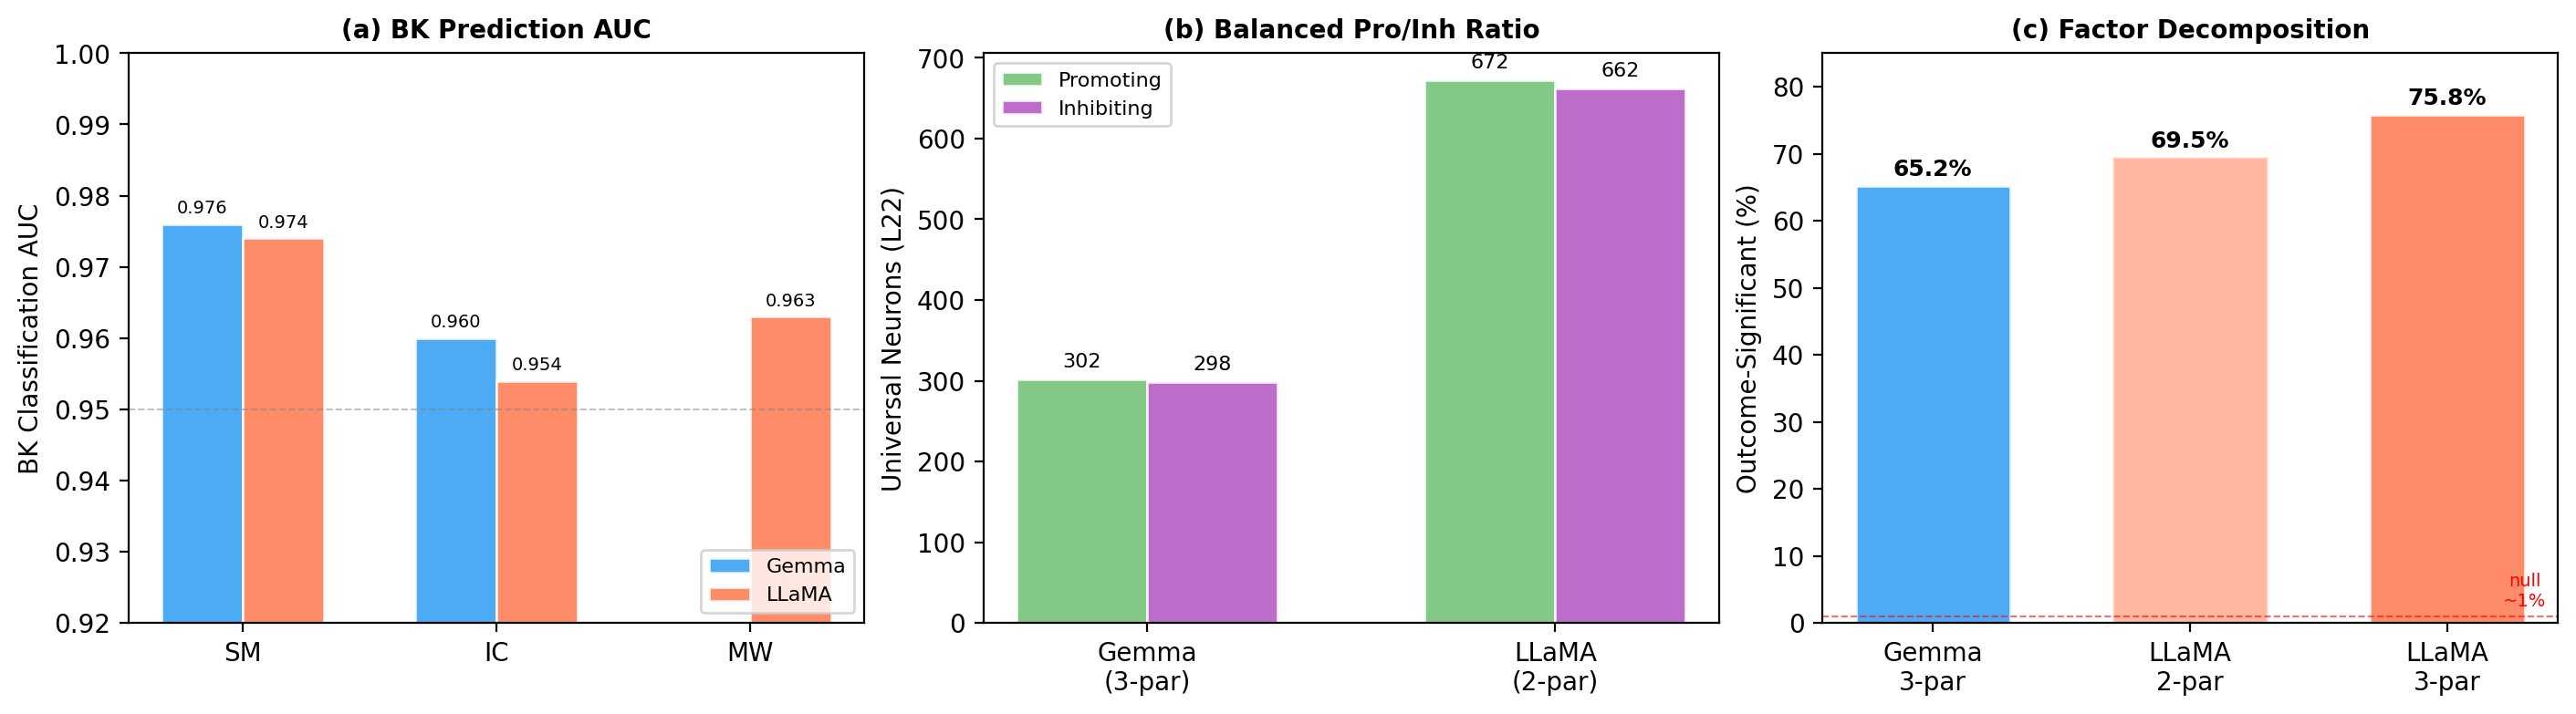
\includegraphics[width=\textwidth]{figures/v10_fig1_rq1_overview.png}
\caption{(a) 교차 모델 BK 분류 AUC. (b) 보편적 BK 뉴런: 촉진/억제 균형 비율. (c) 요인 분해: 결과-유의 65--76\% vs 귀무 ${\sim}$1\%.}
\label{fig:rq1_overview_ko}
\end{figure}

\subsection{RQ1 요약}

BK 예측 정확도는 아키텍처 간에 동등하다 (AUC 차이 $\leq$ 0.006). 두 모델 모두 균형 잡힌 촉진/억제 뉴런 구조를 유지한다. SAE 특징의 65--76\%가 교란 변수와 무관하게 BK를 인코딩한다. 이 세 관찰은 서로 다른 훈련 데이터와 모델 크기에도 불구하고 두 아키텍처에서 공유된 BK 표상이 발생함을 시사한다.

\bigskip\hrule\bigskip

% ============================================================
% 3. RQ2
% ============================================================
\section{RQ2: 도메인이 바뀌어도 BK 패턴이 유지되는가?}

\subsection{교차 도메인 전이}

\begin{table}[H]
\centering
\caption{Gemma SAE 전이 (최적 층)}
\begin{tabular}{lcc}
\toprule
\textbf{전이} & \textbf{AUC} & \textbf{$p$} \\
\midrule
IC $\rightarrow$ MW & 0.932 & 0.000 \\
IC $\rightarrow$ SM & 0.913 & 0.000 \\
SM $\rightarrow$ MW & 0.867 & 0.000 \\
MW $\rightarrow$ IC & 0.853 & 0.000 \\
SM $\rightarrow$ IC & 0.646 & 0.000 \\
\bottomrule
\end{tabular}
\end{table}

\begin{table}[H]
\centering
\caption{LLaMA 3-패러다임 전이 (최적 층)}
\begin{tabular}{lcc}
\toprule
\textbf{전이} & \textbf{AUC} & \textbf{$p$} \\
\midrule
MW $\rightarrow$ IC & 0.805 & 0.000 \\
SM $\rightarrow$ IC & 0.749 & 0.000 \\
IC $\rightarrow$ MW & 0.680 & 0.000 \\
MW $\rightarrow$ SM & 0.682 & 0.000 \\
IC $\rightarrow$ SM & 0.577 & 0.000 \\
\bottomrule
\end{tabular}
\end{table}

두 모델 모두 MW와 관련된 전이에서 강한 성능을 보이며 (AUC 0.68--0.93), IC$\leftrightarrow$SM 전이는 상대적으로 약하고 층에 따라 달라진다. MW는 ``허브(hub)'' 패러다임으로 기능한다: MW에서 학습되거나 MW에 적용되는 BK 패턴이 다른 도메인으로 잘 전이된다.

\begin{figure}[H]
\centering
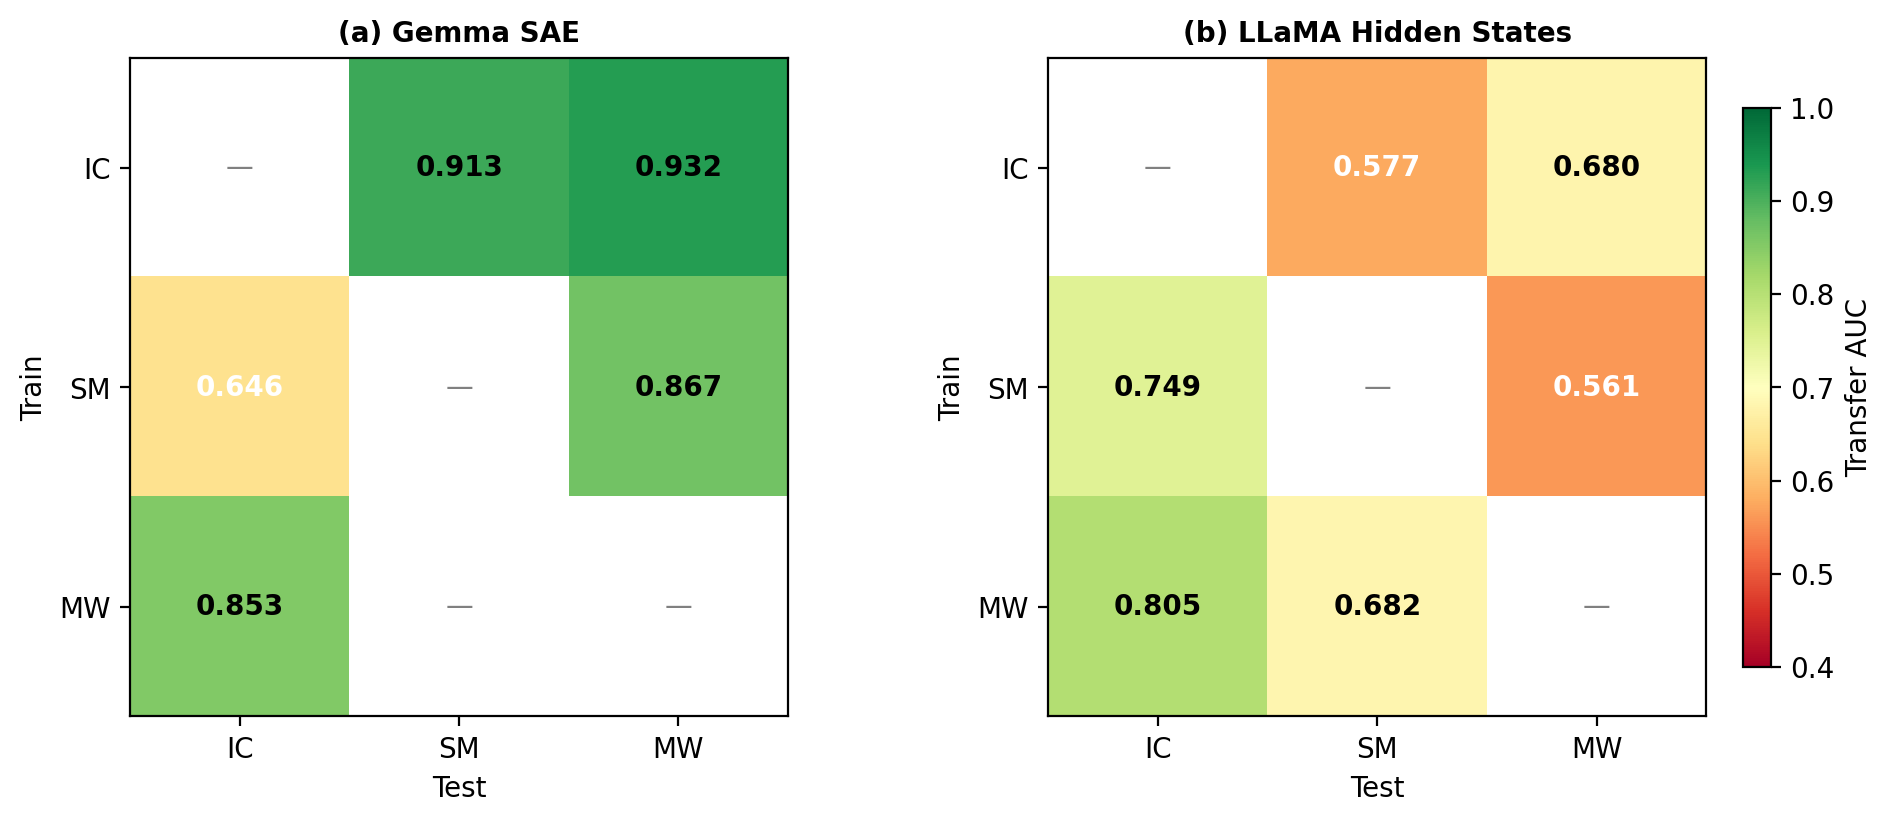
\includegraphics[width=\textwidth]{figures/v10_fig2_rq2_transfer.png}
\caption{교차 도메인 전이 히트맵. (a) Gemma SAE. (b) LLaMA 은닉 상태. 녹색 = 높은 전이; 노란색/빨간색 = 약한 전이.}
\label{fig:rq2_transfer_ko}
\end{figure}

\subsection{공유 BK 부분공간 (Shared BK Subspace)}

패러다임별 분류기의 가중치 벡터는 거의 직교하지만 (코사인 $\approx$ 0.04), 이 가중치 벡터에 PCA를 적용하여 추출한 저차원 부분공간은 높은 AUC를 달성한다.

\begin{table}[H]
\centering
\caption{공유 부분공간 성능}
\begin{tabular}{lcc}
\toprule
 & \textbf{Gemma (3D)} & \textbf{LLaMA (2D)} \\
\midrule
IC AUC & 0.862 & 0.901 \\
SM AUC & 0.899 & 0.943 \\
MW AUC & 0.970 & --- \\
가중치 코사인 & ${\sim}$0.04 & 0.038 \\
\bottomrule
\end{tabular}
\end{table}

거의 직교하는 가중치 벡터에도 불구하고 높은 부분공간 AUC를 달성한다는 것은, BK 신호가 단일 축이 아닌 다차원 부분공간에 분산되어 있음을 의미한다.

\subsection{은닉 상태 vs SAE의 전이 성능}

대부분의 교차 도메인 전이 방향에서 은닉 상태가 SAE보다 우수하다 (Gemma IC$\rightarrow$SM: +0.247; SM$\rightarrow$MW: +0.101; LLaMA SM$\rightarrow$IC: +0.064). SAE 희소화(sparsification)는 교차 도메인 일관성을 잃을 수 있으며, 이는 BK 신호가 희소 분해가 버리는 분산된 저진폭 활성화에 부분적으로 의존함을 시사한다.

\subsection{RQ2 요약}

교차 도메인 전이는 두 모델 모두에서 성공한다 (AUC 0.58--0.93, 모두 $p$=0.000). MW가 가장 강력한 허브 패러다임이다. 직교 가중치 벡터에도 불구하고 공유 저차원 부분공간이 BK를 포착한다. BK 인코딩은 심층에서 도박 도메인 간에 일반화된다.

\bigskip\hrule\bigskip

% ============================================================
% 4. RQ3
% ============================================================
\section{RQ3: 베팅 조건이 바뀌어도 BK 패턴이 유지되는가?}

\subsection{교차 베팅 유형 전이 (F1)}

고정 베팅 게임에서만 훈련된 BK 분류기를 가변 베팅 게임에 적용하며, 그 반대도 수행한다.

\begin{table}[H]
\centering
\caption{LLaMA IC 은닉 상태 전이}
\begin{tabular}{lccc}
\toprule
\textbf{층} & \textbf{Fix$\rightarrow$Var AUC} & \textbf{Var$\rightarrow$Fix AUC} & \textbf{양방향 $p$} \\
\midrule
L8 & 0.872 & 0.842 & 0.000 \\
L12 & 0.772 & 0.927 & 0.000 \\
L22 & 0.736 & 0.912 & 0.000 \\
L30 & 0.819 & 0.911 & 0.000 \\
\bottomrule
\end{tabular}
\end{table}

\begin{table}[H]
\centering
\caption{Gemma IC SAE 전이}
\begin{tabular}{lccc}
\toprule
\textbf{층} & \textbf{Fix$\rightarrow$Var AUC} & \textbf{Var$\rightarrow$Fix AUC} & \textbf{양방향 $p$} \\
\midrule
L18 & 0.808 & 0.726 & 0.000 \\
L30 & 0.902 & 0.696 & 0.000 \\
L10 & NS & NS & --- \\
\bottomrule
\end{tabular}
\end{table}

LLaMA에서는 모든 층과 양방향 모두 $p$=0.000을 산출한다. Var$\rightarrow$Fix 전이 (0.84--0.93)가 Fix$\rightarrow$Var (0.74--0.87)보다 일관되게 강한데, 이는 가변 게임이 고정 BK 영역을 포괄하는 더 넓은 활성화 공간을 탐색하기 때문일 수 있다. Gemma에서는 심층(L30: Fix$\rightarrow$Var 0.902)이 성공하는 반면, 얕은 층(L10)은 실패한다---교차 조건 전이가 심층 표상을 요구한다는 일반적 패턴과 일치한다. Gemma IC에는 가변 BK 사례가 14개뿐이어서, Gemma 특정 베팅 유형 분석의 통계적 검정력이 제한됨에 유의한다.

\begin{figure}[H]
\centering
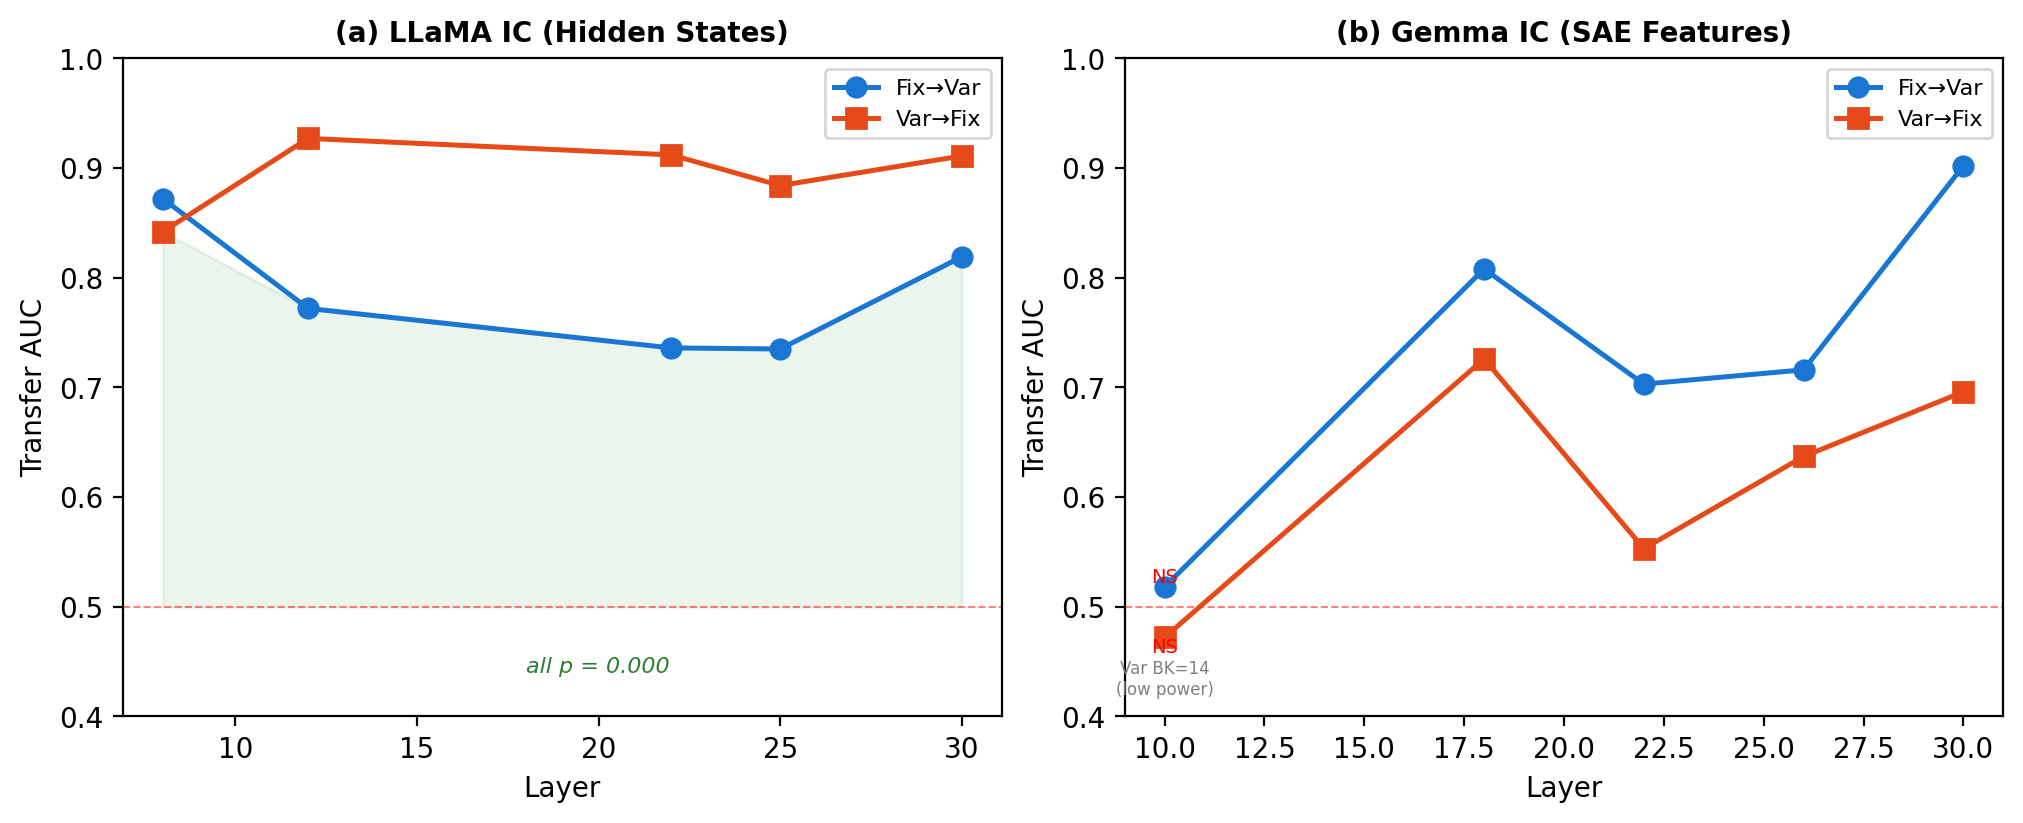
\includegraphics[width=\textwidth]{figures/v10_fig3_rq3_bettype_transfer.png}
\caption{교차 베팅 유형 전이. (a) LLaMA: 모든 층, 양방향, 모두 $p$=0.000. (b) Gemma SAE: 심층 성공; L10 실패.}
\label{fig:rq3_bettype_ko}
\end{figure}

\subsection{방향 코사인과 공통 특징}

가변 BK 방향과 고정 BK 방향 간의 코사인 유사도(cosine similarity)는 보완적 증거를 제공한다. LLaMA IC는 모든 은닉 상태 층에서 $\cos > 0.81$이고, SAE 수준에서 $\cos$ 0.77--0.85이다. Gemma IC는 얕은 층의 음수에서 L30의 $\cos$ ${\sim}$0.39로 수렴한다---가변 BK 표본 크기($n$=14)가 작아 약한 수치를 보인다.

SAE L22에서 415개 LLaMA 특징(및 35개 Gemma 특징)이 두 베팅 조건 모두에서 $d$$\geq$0.3이고 동일 부호를 보인다. 촉진/억제의 균형 비율(LLaMA: 213/202)은 \S2.2의 보편적 뉴런 구조를 반영한다.

\begin{figure}[H]
\centering
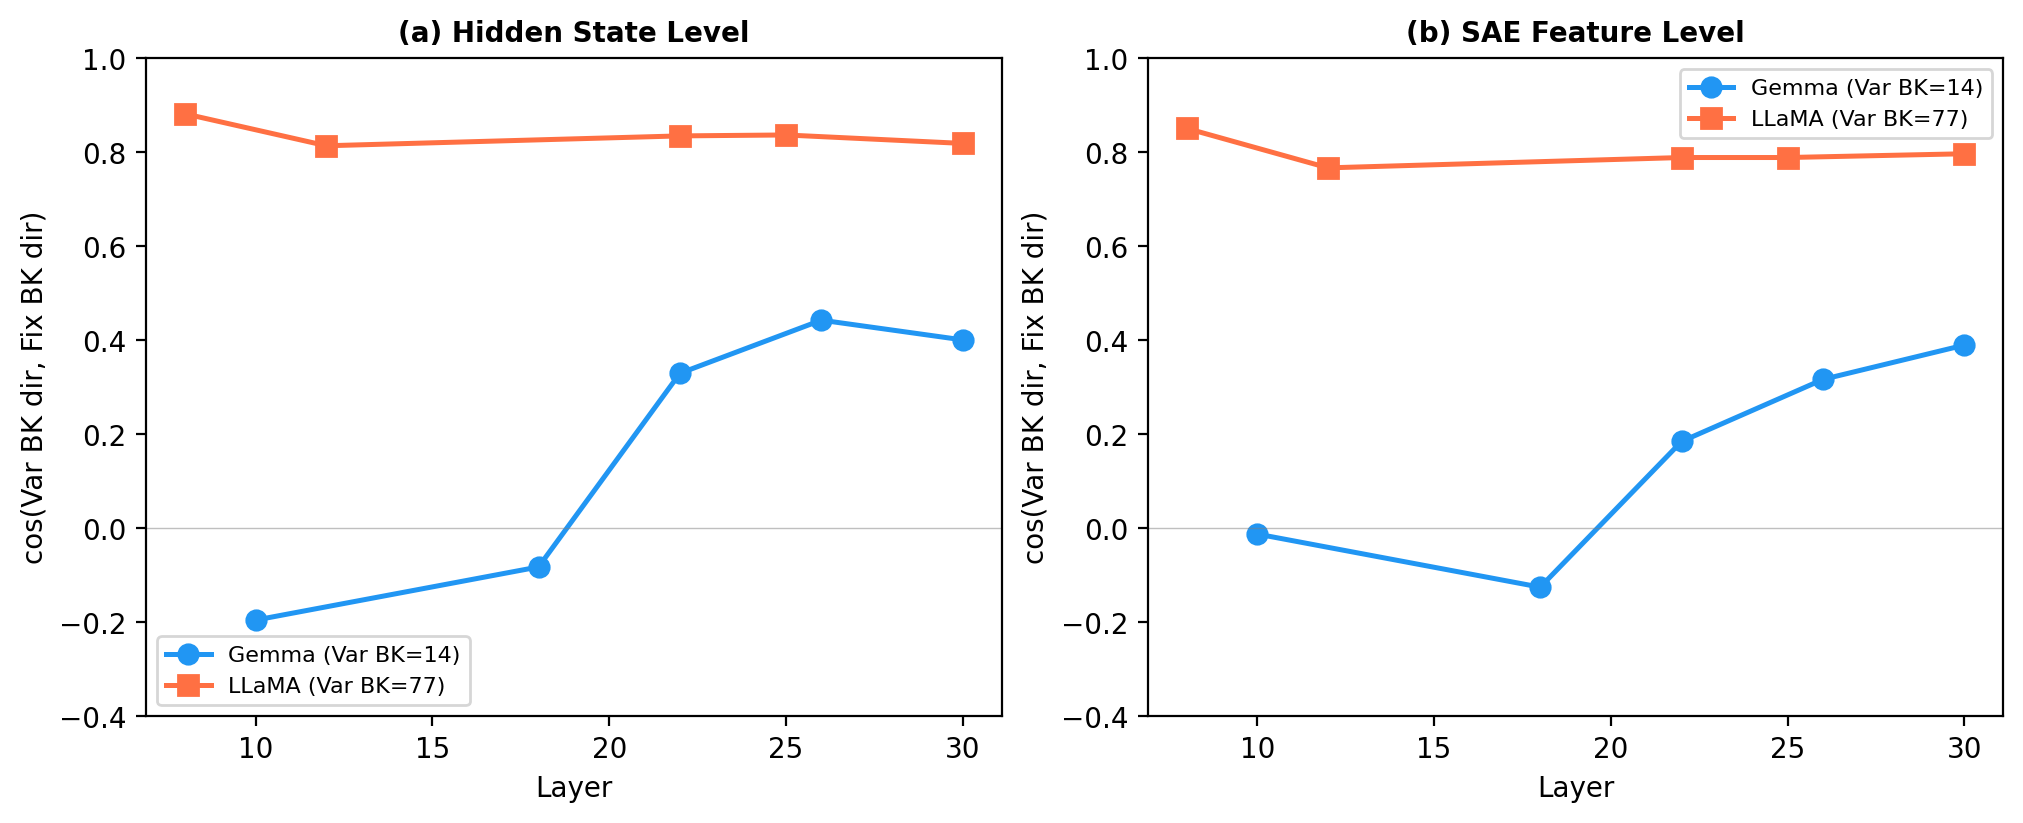
\includegraphics[width=\textwidth]{figures/v10_fig4_rq3_direction_cosine.png}
\caption{가변/고정 방향 코사인: (a) 은닉 상태, (b) SAE 수준. LLaMA $\cos$>0.77 (모든 층); Gemma는 심층에서 수렴.}
\label{fig:rq3_cosine_ko}
\end{figure}

\subsection{G-프롬프트와 베팅 제약 효과}

G(목표 설정) 프롬프트는 두 모델 모두에서 활성화를 BK 방향으로 이동시킨다 ($\cos$ = +0.85 Gemma SM, +0.63 LLaMA SM, L22). 베팅 제약(c10$\rightarrow$c70)은 BK 확률에 선형으로 매핑된다 (Gemma $r$=0.979, LLaMA $r$=0.987; 단 $n$=4 데이터 포인트로 이 선형 주장의 강도가 제한됨에 유의). 이 관찰들은 BK 표상이 이진적 BK/Safe 구분이 아닌 연속적 위험 크기(continuous risk magnitude)를 인코딩함을 시사한다.

\subsection{RQ3 요약}

F1 교차 베팅 유형 전이 분석은 고정과 가변 베팅 조건이 심층에서 동일한 기저 BK 표상을 공유한다는 직접적 증거를 제공한다. 방향 코사인, 공통 특징, G-프롬프트 정렬이 모두 같은 방향을 가리킨다. BK 인코딩은 두 모델 모두에서 고정/가변 조작에 강건하다.

\bigskip\hrule\bigskip

% ============================================================
% 5. 논문 함의
% ============================================================
\section{NMT 논문 \S3.2에 대한 함의}

논문의 \S3.2는 활성화 패칭(activation patching)을 통해 LLaMA SM에서 112개의 인과적 특징을 식별하며, 안전 특징은 L4--L19에, 위험 특징은 L24+ 이상에 위치한다. 본 분석은 그 단일 모델, 단일 도메인 발견을 세 가지 방향으로 확장한다:

\textbf{교차 모델}: Gemma는 거의 동일한 BK 분류를 달성하고 (0.976 vs 0.974) 동일한 균형 촉진/억제 뉴런 구조를 보인다. 112개 인과적 특징은 LLaMA 고유가 아닌 두 아키텍처 모두에 존재하는 속성을 반영할 가능성이 높다.

\textbf{교차 도메인}: BK 분류기가 IC, SM, MW 간에 AUC 최대 0.932로 전이된다. 요인 분해는 특징의 65--76\%가 패러다임과 무관하게 BK를 인코딩함을 보여준다. SM에서 식별된 인과적 특징은 다른 도박 도메인으로 일반화될 가능성이 높다.

\textbf{교차 조건}: 교차 베팅 유형 전이(AUC 0.74--0.93)는 BK 표상이 고정/가변 조작에 강건함을 입증한다---이 조작은 논문의 핵심 행동 발견(가변 베팅이 파산을 증가시킴)을 생성하는 것과 동일하다. 행동 결과가 발산하더라도 신경 표상은 안정적으로 유지된다.

\textbf{인과적 증거}: L22에서의 방향 조향이 유의한 용량-반응을 생성하며 (Spearman $\rho$=0.927, $p$=0.003), 분류를 통해 식별된 BK 방향 벡터가 도박 행동에 인과적 영향을 미침을 확인한다. 이는 V10의 상관적 증거와 논문의 활성화 패칭 결과 사이의 간극을 연결한다.

\bigskip\hrule\bigskip

% ============================================================
% 6. 강건성 검증
% ============================================================
\section{강건성 검증}\label{sec:robustness_ko}

본 절은 \S2--\S4의 분류 결과가 특정 PCA 차원 수나 분류기 알고리즘 선택의 인위적 산물이 아님을 검증한다. PCA 차원 민감도와 분류기 비교의 두 분석으로 이를 다룬다.

\subsection{PCA 차원 민감도}

본 분석의 목적은 보고서 전반에 사용된 PCA=50이 강건한 선택인지, 아니면 결과를 왜곡하는 국소 최적값(local optimum)인지를 판별하는 것이다. 6개 PCA 차원 \{10, 20, 50, 100, 200, Full (PCA 미적용)\}을 6개 모델--패러다임 조합 전체에서 검정했다.

\begin{table}[H]
\centering
\caption{PCA 차원 민감도: PCA=50 vs Full (PCA 미적용) AUC}
\begin{tabular}{lccc}
\toprule
\textbf{데이터셋} & \textbf{PCA=50} & \textbf{Full} & \textbf{50에서 포화?} \\
\midrule
Gemma SM & 0.9755 & 0.9600 & 예 \\
Gemma IC & 0.9568 & 0.9635 & 예 \\
Gemma MW & 0.9658 & 0.9132 & 아니오 (PCA50 > Full) \\
LLaMA SM & 0.9607 & 0.9631 & 예 \\
LLaMA IC & 0.9428 & 0.9195 & 아니오 (PCA50 > Full) \\
LLaMA MW & 0.9590 & 0.9561 & 예 \\
\bottomrule
\end{tabular}
\end{table}

6개 데이터셋 중 4개에서 AUC가 PCA=50 이전 또는 그 지점에서 포화되어, 추가 차원이 의미 있는 판별 정보를 기여하지 않는다. 나머지 2개 데이터셋---Gemma MW와 LLaMA IC---에서는 PCA=50이 전체 차원 표상보다 우수하다. 이 두 데이터셋은 각 모델에서 가장 작은 BK 표본 크기를 가지며 (Gemma MW: $n$=54, LLaMA IC: $n$=142), 고차원 특징 공간이 과적합에 가장 취약한 경우이다. PCA 차원 축소는 이러한 저-$n$ 환경에서 암묵적 정규화기(implicit regularizer)로 작용한다.

전체 패턴은 PCA=50이 강건한 기본값임을 확인한다: 검정한 모든 데이터셋에서 전체 차원 성능과 일치하거나 이를 초과한다.

\subsection{분류기 비교}

본 분석의 목적은 BK 표상이 선형 분리 가능한지, 아니면 비선형 분류기가 추가 신호를 추출하는지를 판별하는 것이다. PCA=50에서 세 분류기를 비교했다: 로지스틱 회귀(LR), 다층 퍼셉트론(MLP), RBF 커널 SVM(SVM-RBF).

\begin{table}[H]
\centering
\caption{분류기 비교: PCA=50에서의 AUC}
\begin{tabular}{lcccc}
\toprule
\textbf{데이터셋} & \textbf{LR} & \textbf{MLP} & \textbf{SVM-RBF} & \textbf{최대 차이} \\
\midrule
Gemma SM & 0.974 & 0.972 & 0.979 & 0.007 \\
Gemma IC & 0.956 & 0.954 & 0.956 & 0.002 \\
Gemma MW & 0.968 & 0.961 & 0.967 & 0.007 \\
LLaMA SM & 0.961 & 0.961 & 0.961 & 0.000 \\
LLaMA IC & 0.940 & 0.945 & 0.942 & 0.005 \\
LLaMA MW & 0.959 & 0.956 & 0.959 & 0.003 \\
\bottomrule
\end{tabular}
\end{table}

6개 데이터셋 모두 세 분류기 간 최대 AUC 차이가 0.01 미만이다. 특정 분류기가 일관되게 우세하지 않는다. Table~11은 BK와 Safe 활성화 상태가 PCA 축소 공간에서 선형 분리 가능함을 입증한다: 비선형 결정 경계(MLP, SVM-RBF)는 선형 초평면(로지스틱 회귀)에 비해 체계적 이점을 제공하지 않는다.

\subsection{강건성 요약}

PCA=50은 대부분의 데이터셋에서 AUC를 포화시키고, 저-$n$ 데이터셋에서 과적합을 방지하는 강건한 선택이다. 로지스틱 회귀는 BK 분류에 충분하며, 이는 BK 표상이 선형 분리 가능하기 때문이다. 이 결과들은 \S2--\S4의 발견이 파이프라인 하이퍼파라미터의 인위적 산물이 아님을 확인한다.

\bigskip\hrule\bigskip

% ============================================================
% 7. 인과적 검증
% ============================================================
\section{인과적 검증: BK 방향 조향}\label{sec:steering_ko}

V10은 두 모델이 BK를 1{,}334개(LLaMA) 및 600개(Gemma)의 보편적 뉴런을 통해 인코딩하며, 높은 분류 AUC와 교차 도메인 전이를 보임을 확립했다. 그러나 V10의 모든 증거는 상관적이다. 본 절은 BK 방향 벡터가 도박 행동을 인과적으로 통제하는지를 검정한다.

\subsection{뉴런 수준 제거 (영 결과)}

본 분석의 목적은 특정 뉴런이 BK 행동을 구동한다는 가장 단순한 인과적 가설을 검정하는 것이다. \S2.2에서 식별한 104개 강한 촉진 뉴런과 89개 강한 억제 뉴런(LLaMA, L22)에 영 제거(zero ablation)를 적용했다. 각 조건은 50개 SM 게임에서 검정되었다.

어떤 조건도 유의한 행동 변화를 보이지 않았다 (Fisher 정확 검정, 모든 $p$ > 0.5). 무작위 뉴런 통제(동일 수의 무작위 선택 뉴런)도 효과가 없었다. 이 영 결과는 BK 행동이 개별 뉴런에 집중되어 있다는 가설을 기각한다. 대신, \S2.2에서 식별된 균형 촉진/억제 구조는 BK가 전체 활성화 공간에 걸친 분산 방향(distributed direction)으로 인코딩됨을 시사한다.

\subsection{방향 조향 방법}

BK 방향 벡터는 L22에서 평균 BK 은닉 상태와 평균 Safe 은닉 상태의 차이로 정의되며, LLaMA 활성화 공간에서 4{,}096차원 벡터를 산출한다. 이 벡터를 스케일링 계수 $\alpha \in \{-2, -1, -0.5, 0, 0.5, 1, 2\}$로 L22의 잔차 스트림에 추가했다. 음의 $\alpha$는 표상을 BK에서 멀어지게(Safe 방향으로) 밀고, 양의 $\alpha$는 BK 방향으로 민다. 각 조건은 50개 SM 게임에서 검정했다. 무작위 방향 통제(단위 노름 무작위 벡터)를 $\alpha$=1.0에서 검정했다.

\subsection{조향 결과}

\begin{table}[H]
\centering
\caption{BK 방향 조향 (LLaMA L22, SM, 조건당 $n$=50)}
\begin{tabular}{ccc}
\toprule
\textbf{Alpha} & \textbf{중단율} & \textbf{BK율} \\
\midrule
$-$2.0 & 0.660 & 0.340 \\
$-$1.0 & 0.520 & 0.480 \\
$-$0.5 & 0.580 & 0.420 \\
0 (기준선) & 0.520 & 0.480 \\
$+$0.5 & 0.500 & 0.500 \\
$+$1.0 & 0.480 & 0.520 \\
$+$2.0 & 0.480 & 0.520 \\
무작위 방향 ($\alpha$=1) & 0.660 & 0.340 \\
\bottomrule
\end{tabular}
\end{table}

Table~12는 조향 크기와 BK율 사이의 단조적 관계를 보여준다. $\alpha$가 $-$2에서 $+$2로 증가함에 따라 BK율이 34\%에서 52\%로 증가한다.

\begin{figure}[H]
\centering
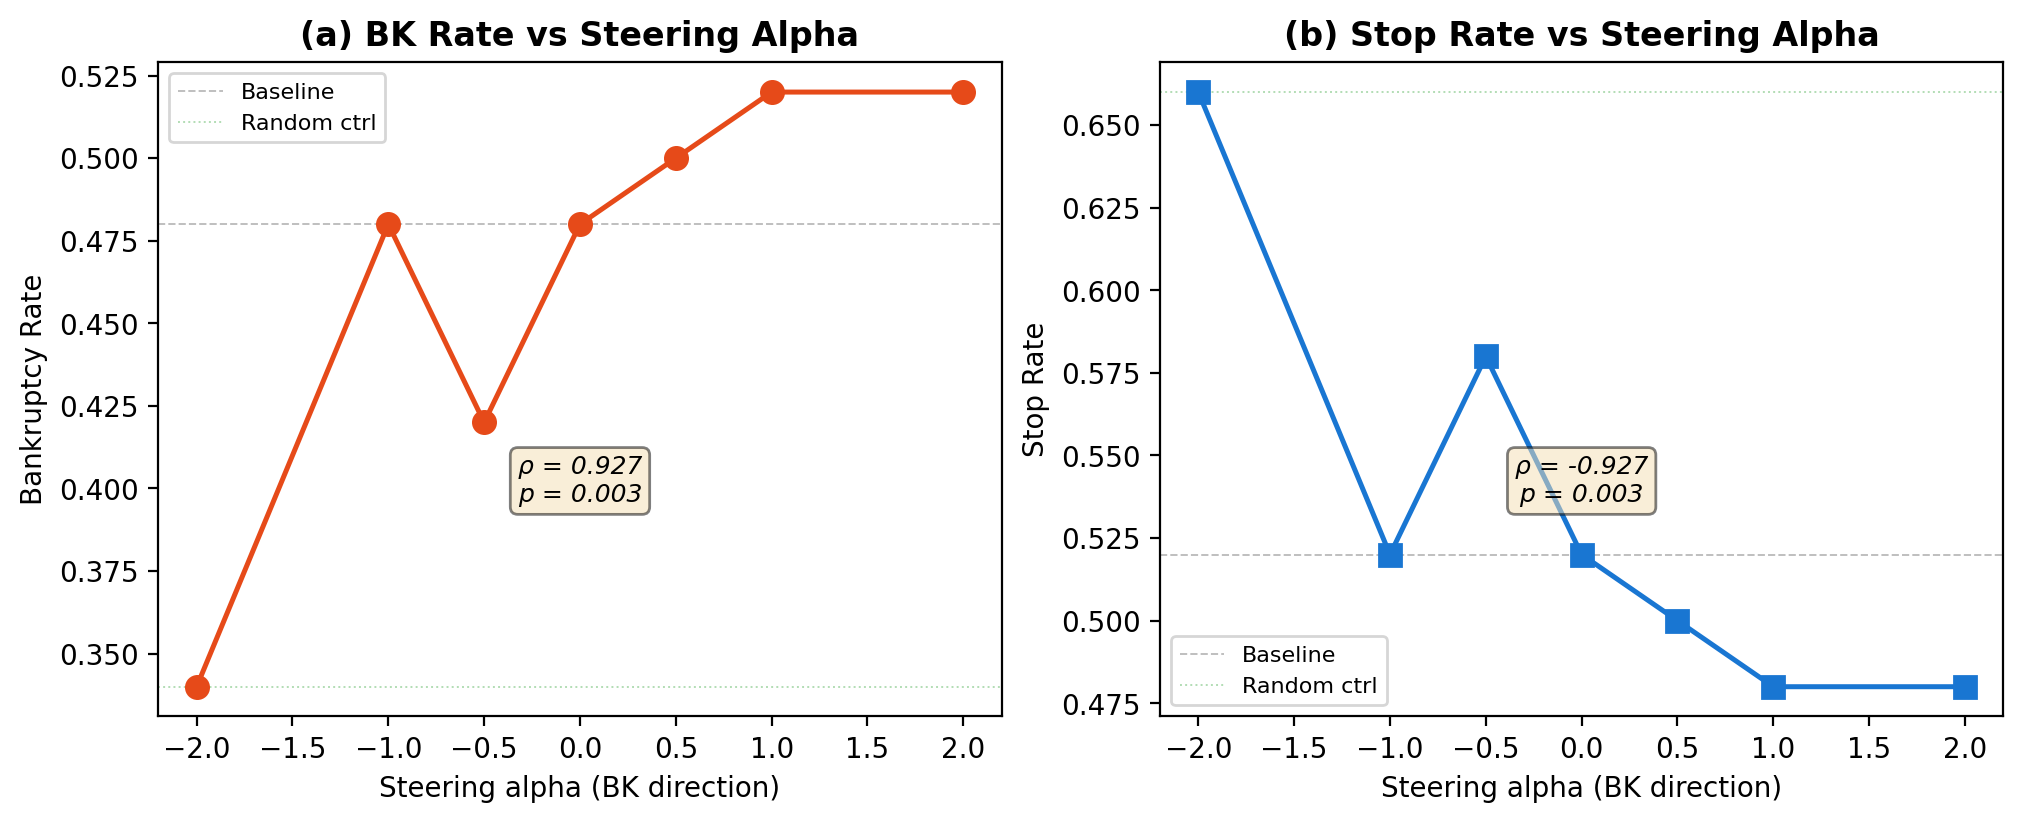
\includegraphics[width=\textwidth]{figures/v11_fig5_steering_doseresponse.png}
\caption{BK 방향 조향 용량-반응. (a) BK율이 $\alpha$와 단조적으로 증가 (Spearman $\rho$=0.927, $p$=0.003). (b) 중단율이 대응적으로 감소. 점선 = 기준선; 점점선 = $\alpha$=1에서의 무작위 방향 통제.}
\label{fig:steering_ko}
\end{figure}

\textbf{Fig.~5 해석}: 용량-반응 곡선은 BK 방향 벡터가 도박 행동에 인과적 영향을 미침을 확인한다. 패널 (a): BK 방향으로 밀면(양의 $\alpha$) 파산이 증가하고, 반대 방향으로 밀면(음의 $\alpha$) 중단이 증가한다. 관계는 단조적이다 (Spearman $\rho$=0.927, $p$=0.003). 패널 (b): 중단율이 이 패턴을 반영한다. 무작위 방향 통제(점점선)는 단일 $\alpha$ 값에서 높은 중단율을 보이지만, BK 방향만이 7개 $\alpha$ 값에 걸친 점진적 용량-반응을 보여준다.

\subsection{무작위 방향 통제와 주의사항}

$\alpha$=1.0에서의 무작위 방향 통제는 중단율 0.660, BK율 0.340을 생성하며, 이는 $\alpha$=$-$2.0에서의 BK 방향과 크기가 비슷하다. 이는 잔차 스트림에 대한 임의의 교란이 보수적 행동(중단)을 증가시키는 경향이 있음을 나타내며, 매니폴드 밖(off-manifold) 교란이 모델의 기본 행동 패턴을 방해하기 때문일 것이다.

BK 방향 조향과 무작위 교란 사이의 결정적 차이는 \textbf{용량-반응 패턴}이다. BK 방향 조향은 7개 $\alpha$ 값에 걸쳐 단조적 $\alpha$--BK 관계를 생성한다 ($\rho$=0.927, $p$=0.003): 더 양의 $\alpha$가 더 많은 파산을 산출한다. 무작위 방향은 단일 $\alpha$ 값($\alpha$=1.0)에서만 검정되었으므로, 용량-반응을 입증하거나 반증할 수 없다. 방향 특이성을 완전히 확립하려면, 무작위 방향 통제를 여러 $\alpha$ 값에서 검정해야 한다. 무작위 방향 조향도 비슷한 기울기의 단조적 용량-반응을 생성한다면, BK 방향은 고유하게 유익하지 않을 수 있다. 예상대로 무작위 방향이 평탄하거나 비단조적 프로필을 생성한다면, 용량-반응 패턴은 BK 방향에 특이적이다.

\subsection{상관적 증거와 인과적 증거의 연결}

조향 결과는 세 수준의 증거를 연결한다:

\begin{enumerate}[nosep]
    \item \textbf{상관적} (\S2--\S4): BK와 Safe 상태가 분류 가능하고 (AUC > 0.95), 도메인 간 전이되며 (AUC 0.58--0.93), 저차원 부분공간을 공유한다.
    \item \textbf{뉴런 수준 인과적} (\S7.1): 개별 뉴런 제거가 효과를 보이지 않아, 희소 인과 메커니즘을 기각한다.
    \item \textbf{방향 수준 인과적} (\S7.3): BK 방향 벡터가 유의한 용량-반응을 생성하며 ($p$=0.003), 분산 BK 표상의 인과적 영향을 확인한다.
\end{enumerate}

상관적 분류에서 인과적 조향으로의 이 진행은 해석 틀을 검증한다: BK는 도박 행동을 예측하고 통제하는 분산적, 방향적 표상이다.

\subsection{인과적 검증 요약}

뉴런 수준 제거는 영 결과를 산출하여, BK가 특정 뉴런에 집중되지 않고 분산되어 있음을 확인한다. 방향 수준 조향은 단조적 용량-반응을 생성하며 (Spearman $\rho$=0.927, $p$=0.003), BK 방향의 도박 행동에 대한 인과적 영향을 확립한다. 무작위 방향 통제 주의사항---임의 교란도 행동을 변화시킨다는 점---은 다중-$\alpha$ 검정으로 해결해야 한다. 용량-반응 패턴이 방향 특이성의 핵심 증거이다.

\bigskip\hrule\bigskip

% ============================================================
% 8. 한계
% ============================================================
\section{한계}

\begin{enumerate}[leftmargin=2em]
    \item \textbf{교차 모델 및 교차 도메인 주장의 상관적 증거.} 방향 조향을 통한 인과적 검증은 LLaMA SM에서만 수행되었다 (\S7). 교차 모델(Gemma) 및 교차 도메인(IC, MW) 인과적 검증은 미완이다.

    \item \textbf{표본 크기 불균형.} Gemma IC는 가변 BK 사례가 14개뿐이어서, Gemma 베팅 유형 분석의 검정력이 심각하게 제한된다. Gemma MW는 54개 BK 사례를 가진다. LLaMA MW는 2{,}426개 BK (75.8\%)---이 높은 기저율에서는 사소한 분류기도 잘 수행하며, 균형 클래스 가중치가 부분적으로 완화하지만 보완 지표(균형 정확도, F1)가 주장을 강화할 것이다.

    \item \textbf{층 범위.} LLaMA 은닉 상태는 32개 중 5개 층(L8, L12, L22, L25, L30)에서 추출된다. 이 체크포인트 사이의 층별 현상을 놓칠 수 있다.

    \item \textbf{베팅 제약 선형성.} $r$=0.979/0.987 선형 매핑은 4개 데이터 포인트(c10, c30, c50, c70)에서만 계산된다. $df$=2이면 무작위 관계도 빈번히 선형으로 나타난다.

    \item \textbf{공통 BK 특징.} 415개 공통 특징($d$$\geq$0.3, 두 베팅 유형 모두 동일 부호)은 순열 귀무 비교가 없다. 우연히 이 기준을 충족하는 특징의 기대 수가 계산되지 않았다.

    \item \textbf{다중 비교.} FDR 보정은 개별 분석 내에서 적용되지만, 전체 분석 세트에 걸쳐 적용되지 않는다. 효과 크기를 주요 증거로 취급해야 한다.

    \item \textbf{두 모델만 검정.} 다른 아키텍처(예: Qwen, Mistral)로의 일반화는 검정되지 않았다.

    \item \textbf{조향 무작위 통제 주의사항.} $\alpha$=1에서의 무작위 방향 교란이 $\alpha$=$-$2에서의 BK 방향과 비슷한 크기의 행동 변화를 생성했다. 용량-반응의 방향 특이성은 무작위 방향을 여러 $\alpha$ 값에서 검정하여 BK 방향이 무작위보다 더 강한 단조적 관계를 생성함을 확인해야 한다.

    \item \textbf{조향 $n$=50.} 각 조향 조건은 50개 게임에서 검정되었다. 더 큰 $n$이 용량-반응 곡선의 정밀도를 개선하고, 중간 $\alpha$ 값에서의 더 작은 효과 크기 탐지를 가능하게 할 것이다.
\end{enumerate}

\bigskip\hrule\bigskip

% ============================================================
% 9. 향후 과제
% ============================================================
\section{향후 과제}

\begin{enumerate}[leftmargin=2em]
    \item \textbf{다중 알파 무작위 방향 통제}: 무작위 방향을 $\alpha \in \{-2, -1, -0.5, 0.5, 1, 2\}$에서 검정하여, BK 방향이 무작위 교란보다 더 강한 용량-반응을 생성하는지 확인한다.
    \item \textbf{다중 층 조향}: L22 + L25 + L30 동시 조향으로 다중 층 개입이 용량-반응 효과를 증폭하는지 검정한다.
    \item \textbf{Gemma 조향 복제}: BK 방향 조향을 Gemma에 적용하여 교차 모델 인과적 일반화를 검정한다.
    \item \textbf{415개 공통 특징의 순열 귀무}: 레이블 순열 하에서 두 베팅 유형 모두 $d$$\geq$0.3인 특징의 기대 수를 계산하여, 415가 우연을 초과하는지 확인한다.
\end{enumerate}

\end{document}
